%% For double-blind review submission
%\documentclass[sigplan,10pt]{acmart}
\documentclass[sigconf]{acmart}
\settopmatter{printfolios=true}
%% For final camera-ready submission
%\documentclass[acmlarge]{acmart}\settopmatter{}

\makeatletter\if@ACM@journal\makeatother

%% Journal information (used by PACMPL format)
%% Supplied to authors by publisher for camera-ready submission
\acmJournal{PACMPL}
\acmVolume{1}
\acmNumber{1}
\acmArticle{1}
\acmYear{2018}
\acmMonth{1}
\acmDOI{10.1145/nnnnnnn.nnnnnnn}
\startPage{1}
\else\makeatother

%% Conference information (used by SIGPLAN proceedings format)
%% Supplied to authors by publisher for camera-ready submission
\acmConference[SBLP'18]{XXII Brazilian Symposium on Programming Languages}{2018}{Brasil}
\acmYear{2018}
\acmISBN{978-1-4503-6480-5/18/09}
\acmDOI{10.1145/nnnnnnn.nnnnnnn}
\startPage{1}
\fi

\newcommand{\fer}[1]{\textcolor{red}{#1}}

%% For review submission
\setcopyright{none}

%% Bibliography style
\bibliographystyle{ACM-Reference-Format}
%\citestyle{acmauthoryear}

%% Packages that we are using in this version of the work:
\usepackage{amsmath}
\usepackage{hyperref}
\usepackage{paralist}
\usepackage[brazil]{babel}
\usepackage[utf8]{inputenc}
\usepackage{mathpartir}


% To turn comments OFF simply comment out the \Commentstrue line
\newif\ifComments\Commentstrue

\ifComments
\newcommand{\marcio}[1]{\noindent\textcolor{violet}{Marcio: {#1}}}
\newcommand{\guido}[1]{\noindent\textcolor{magenta}{Guido: {#1}}}
\newcommand{\fernando}[1]{\noindent\textcolor{brown}{Fernando: {#1}}}
\newcommand{\cesar}[1]{\noindent\textcolor{magenta}{Cesar: {#1}}}
\newcommand{\pedro}[1]{\noindent\textcolor{brown}{Pedro: {#1}}}
\newcommand{\rmv}[1]{\noindent\textcolor{gray}{Removed: {#1}}}
\newcommand{\new}[1]{\noindent\textcolor{blue}{ {#1}}}
\newcommand{\ed}[1]{\noindent\textcolor{red}{ {#1}}}
\else
\newcommand{\marcio}[1]{}
\newcommand{\guido}[1]{}
\newcommand{\fernando}[1]{}
\newcommand{\cesar}[1]{}
\newcommand{\pedro}[1]{}
\newcommand{\rmv}[1]{}
\newcommand{\new}[1]{#1}
\newcommand{\ed}[1]{}
\fi
\newcommand\dawn{\mbox{\textsf{DawnCC}}}
\newcommand\Taskminer{\mbox{\textsf{TaskMiner}}}

\newtheorem{Challenge}{Challenge}[section]
\newtheorem{Definicao}{Defini\c{c}\~{a}o}

\begin{document}

\title[TaskMiner: Identifica\c{c}\~{a}o Autom\'{a}tica de Tarefas]
{TaskMiner: Identificação Automática de Tarefas}



\author{Pedro Ramos, Gleison Souza, Guilherme Leobas, Fernando Magno Quint\~{a}o Pereira}
%\authornote{with author1 note}          %% \authornote is optional;
%\orcid{nnnn-nnnn-nnnn-nnnn}
\affiliation{
  %\position{Researcher}
  %\department{DCC}
  \institution{UFMG}
%  \streetaddress{6627 Antonio Carlos Avenue}
%  \city{Belo Horizonte}
%  \state{Minas Gerais}
 % \postcode{31.270-213}
 % \country{Brazil}
}
\email{[pedroramos, gleison.mendonca, guilhermel, fernando]@dcc.ufmg.br}

%\author{Gleison Souza Diniz Mendonc\c{c}a}
%\authornote{with author1 note}          %% \authornote is optional;
%\orcid{nnnn-nnnn-nnnn-nnnn}
%\affiliation{
 % \position{Researcher}
%  \department{DCC}
 % \institution{UFMG}
 % \streetaddress{6627 Antonio Carlos Avenue}
%  \city{Belo Horizonte}
%  \state{Minas Gerais}
%  \postcode{31.270-213}
%  \country{Brazil}
%}
%\email{gleison.mendonca@dcc.ufmg.br}

%\author{Guilherme Mendes Leobas}
%\authornote{with author1 note}          %% \authornote is optional;
%\orcid{nnnn-nnnn-nnnn-nnnn}
%\affiliation{
%  \position{Researcher}
%  \department{DCC}
%  \institution{UFMG}
%  \streetaddress{6627 Antonio Carlos Avenue}
%  \city{Belo Horizonte}
%  \state{Minas Gerais}
%  \postcode{31.270-213}
%  \country{Brazil}
%}
%\email{guihermel@dcc.ufmg.br}

%\author{Fernando M Q Pereira}
%\authornote{with author1 note}
%\orcid{nnnn-nnnn-nnnn-nnnn}
%affiliation{
 % \position{Professor}
 % \department{DCC}
 % \institution{UFMG}
 % \streetaddress{6627 Antonio Carlos Avenue}
 % \city{Belo Horizonte}
 % \state{Minas Gerais}
 % \postcode{31.270-213}
 % \country{Brazil}
%}
%\email{fernando@dcc.ufmg.br}          %% \email is recommended

\begin{abstract}
Este artigo apresenta \Taskminer{}, uma ferramenta que encontra paralelismo de tarefas
em código C automaticamente. \Taskminer{} lida com problemas clássicos de paralelismo irregular 
como a delimitação simbólica de regiões de memória, remoção de dependências
estáticas espúrias, detecção de condições de corrida, e, principalmente, a avaliação do custo do paralelismo. Para solucioná-los,
\Taskminer{} implementa uma série de otimizações em representa\-ção intermedi-ária do LLVM, que analisam código C e inserem anotações OpenMP automaticamente. \Taskminer{} prova-se eficaz ao encontrar paralelismo apontado manualmente em benchmarks como \textsf{BSC-Bots}~\cite{Duran09}, produzindo programas tão rápidos ou mais velozes que as versões sequenciais e anotadas manualmente. \Taskminer{} também é capaz de encontrar paralelismo escondido em programas sequenciais, sem intervenção humana.
\end{abstract}

%% 2012 ACM Computing Classification System (CSS) concepts
%% Generate at 'http://dl.acm.org/ccs/ccs.cfm'.
\begin{CCSXML}
<ccs2012>
<concept>
<concept_id>10010520.10010521.10010528</concept_id>
<concept_desc>Computer systems organization~Parallel architectures</concept_desc>
<concept_significance>500</concept_significance>
</concept>
<concept>
<concept_id>10010520.10010521.10010528.10010536</concept_id>
<concept_desc>Computer systems organization~Multicore architectures</concept_desc>
<concept_significance>100</concept_significance>
</concept>
<concept>
<concept_id>10011007.10011006.10011041</concept_id>
<concept_desc>Software and its engineering~Compilers</concept_desc>
<concept_significance>500</concept_significance>
</concept>
<concept>
<concept_id>10011007.10011006.10011041.10011047</concept_id>
<concept_desc>Software and its engineering~Source code generation</concept_desc>
<concept_significance>300</concept_significance>
</concept>
</ccs2012>
\end{CCSXML}

\ccsdesc[500]{Computer systems organization~Parallel architectures}
\ccsdesc[500]{Software and its engineering~Compilers}
\ccsdesc[300]{Software and its engineering~Source code generation}

\keywords{paralelismo, tarefas, OpenMP, compiladores}

\maketitle

\section{Introdu\c{c}\~{a}o}
\label{sec:intro}

É inegável que computação paralela e distribuída é hoje uma alternativa muito procurada por 
desenvolvedores na busca por desempenho. Programadores tem, cada vez mais, investido
em paradigmas paralelos visando maior eficiência e velocidade. Nesse contexto, sistemas de
anotação como OpenMP~\cite{JaegerCP15} e
OpenACC~\cite{OpenACC20} atuam como metalinguagens, conferindo ao programador
poder semântico para transformar um programa originalmente sequencial
em um programa paralelo. Tais sistemas mostram-se muito promissores quando
combinados com aceleradores como GPUs e FPGAs~\cite{Mendonca17,Poesia17}.
Entretanto, apesar de conveniente, o uso desses sistemas não é automático e
requer exaustiva escrutinação de olho humano para garantia de corretude e eficiência.

Embora existam ferramentas que anotem programas automaticamente~\cite{Mendonca16,Pingali11},
essas tecnologias exploram somente paralelismo de dados.  Porém, grande
parte do poder de sistemas de anotação provém da capacidade de se criar \textit{tarefas}
durante a execução do programa~\cite{Ayguade09}. O propósito desse trabalho
é apresentar um algoritmo capaz de minerar oportunidades para paralelismo de tarefas
em programas sequênciais e anotá-los automaticamente. Como descrito na seção \ref{sec:ovf},
essas anotações conferem ao programa irregular uma semântica de paradigmas paralelos,
como aqueles em grafos e/ou em \textit{worklists}~\cite{Pingali11}.

Este artigo descreve {\Taskminer}, um compilador fonte-a-fonte que expõe
paralelismo de tarefas em programas C/C++. {\Taskminer} lida com desafios 
relacionados ao paralelismo irregular. Primeiro, ele determina os limites
simbólicos dos blocos de memória acessados dentro de cada programa. Depois, encontra 
fragmentos de código (laços ou funções) que podem 
ser efetivamente mapeados em tarefas. Então, extrai parâmetros capazes
de estimar o custo da tarefa em questão. Esses parâmetros estão dinamicamente atrelados
às anotações e são capazes de ativar ou desativar a criação de tarefas durante a execução do programa,
ou de limitar a profundidade de tarefas geradas recursivamente. \Taskminer{} também determina
quais variáveis serão replicadas em novas tarefas ou compartilhadas por tarefas concorrentes.
Finalmente, ele mapeia todas essas informações de volta ao código fonte, produzindo
anotações legíveis.

Defende-se a tese de que a anotação automática de tarefas é útil à medida que
retira do programador o fardo de procurar, anotar e verificar as anotações, tornando seu
processo de desenvolvimento mais eficiente. A ferramenta {\Taskminer} é capaz
de alcançar ganhos de quase 4x em benchmarks não usualmente paralelos, como descrito na Seção \ref{sec:eval}. {\Taskminer}
recebe como entrada um programa escrito em C e produz como saída um programa também em C,
mas anotado com diretivas OpenMP legíveis. {\Taskminer} anota programas não triviais, envolvendo
todo tipo de construto da linguagem C, como arranjos, estruturas, uniões e ponteiros para esses tipos.
Alguns desses programas provém de benchmarks complexos como Bots~\cite{Duran09}  e a coleção de testes do LLVM.
As versões anotadas pelo {\Taskminer} se aproximam das versões anotadas manualmente em
desempenho e são mais rápidas que as versões sequenciais.

\Taskminer{} está online e disponível para uso acadêmico em \url{http://cuda.dcc.ufmg.br/taskminer/}.


\section{Visão geral}
\label{sec:ovf}

A construção de um compilador como o \Taskminer{} envolve a supera-ção de uma série  de desafios.
\Taskminer{} recebe como entrada um programa escrito em C e retorna o mesmo programa anotado com 
diretivas OpenMP. O ambiente de execução OpenMP se encarrega de 
rastrear dependências entre ponteiros~\cite{LaGrone11}. Entretanto, a inserção
automática das anotações é apenas a última etapa. Nesta Seção detalham-se os problemas
encontrados pelo \Taskminer{} no percalço de mineração de tarefas. A solução para esses problemas é descrita na Seção~\ref{sec:sol}.

\begin{figure}[b!]
\begin{center}
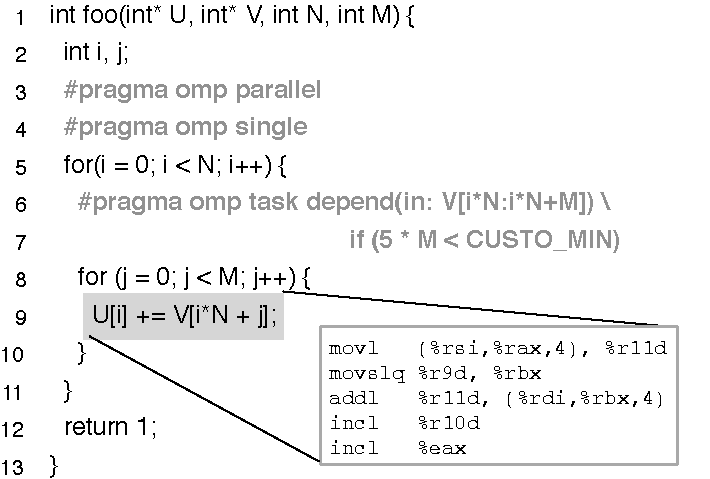
\includegraphics[width=1\columnwidth]{images/ex_Regions}
\caption{Identificando limites de memória e o custo de uma tarefa.}
\label{fig:ex_Regions}
\end{center}
\end{figure}

O primeiro desafio encontrado pelo \Taskminer{} consiste em 
identificar as regiões de memória cobertas por uma tarefa.
A Figura~\ref{fig:ex_Regions} ilustra esse problema e como resolvê-lo. O programa
recebe uma matriz \textsf{V}, $\mathsf{M}\times\mathsf{N}$, em formato linear,
e produz um vetor  \textsf{U} de forma que  \textsf{U[i]} contenha a soma de todos
os elementos na linha  \textsf{i} da matriz  \textsf{V}. {\Taskminer} determina que cada
iteração do laço mais externo pode se tornar uma tarefa. Então, cada tarefa neste programa
consiste no laço mais interno, e atravessa a região de memória entre os endereços  \textsf{\&V + i * N} e
 \textsf{\&V + i * N + M}. A identificação desses limites envolve o uso de álgebra simbólica baseada
 na literatura de compiladores.
 
A Figura~\ref{fig:ex_Regions} apresenta um outro problema: {\em como estimar a rentabilidade de uma tarefa?}
A criação de tarefas envolve um custo alto por parte do ambiente de execução, causado por questões como
alocação, escalonamento, concorrência e gerenciamento em tempo real do grafo de dependências.
Idealmente, são desejáveis tarefas que executem uma quantidade de trabalho
grande o suficiente para superar este custo. A quantidade de trabalho executado
por uma tarefa não pode ser descoberta estaticamente \cite{Rice53}. Contudo,
é possível aproximar-se desse custo com
símbolos nativos do programa, que, em execução, serão substituídos por valores. 
Por exemplo, na Figura~\ref{fig:ex_Regions}
sabe-se o número de instruções do laço interno. Então, aproxima-se a quantidade de trabalho executado
com a expressão \textsf{5 * M}. O valor de \textsf{M} durante a execução será determinante para
a criação da tarefa. Essa checagem é feita na linha 7 do exemplo, 
e faz parte da sintaxe de OpenMP. Além disso, {\Taskminer} propõe
uma estimativa confiável a respeito do limite mínimo de custo 
que uma tarefa deve possuir para ser criada sem produzir
excesso de computação. Esse limite considera fatores como número de 
núcleos disponíveis e informações a respeito do ambiente
de execução em termos de instruções de máquina.
	
\begin{figure}[h!]
\begin{center}
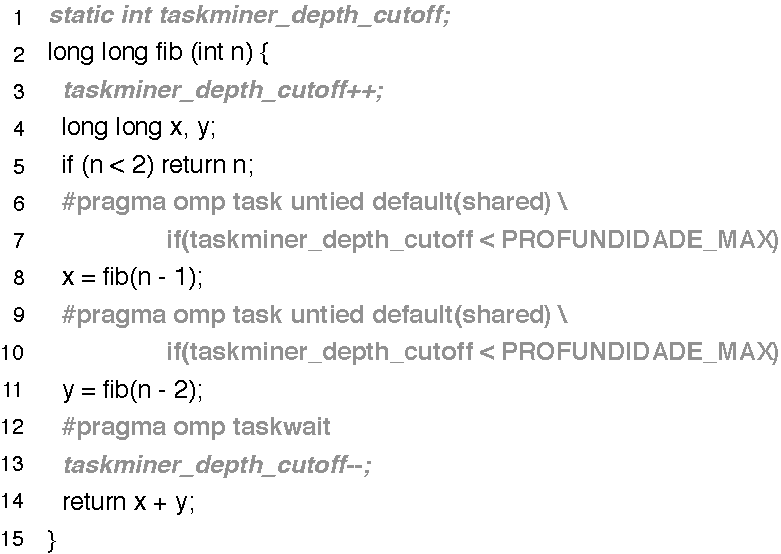
\includegraphics[width=1\columnwidth]{images/ex_cutoff}
\caption{Limitando a criação de tarefas recursivas.
Exemplo retirado de~\cite[Fig.1]{Iwasaki16}.}
\label{fig:ex_cutoff}
\end{center}
\end{figure}
	
No paralelismo de tarefas, um fator importante para bom desempenho
é o uso de cortes mínimos para o número de tarefas a serem criadas~\cite{Duran08b}. 
Observa-se esse fator no contexto de tarefas recursivas. 
Uma variável de controle é inserida no código para controlar
a criação de tarefas de baixa granularidade, como ilustrado na Figura~\ref{fig:ex_cutoff}. 
Um contador é associado à invocação das funções recursivas anotadas como tarefas. 
A checagem na linha 7 certifica-se de que o limite
nunca é excedido. Esse limite é pré-determinado na fase de configuração do 
{\Taskminer}, assim como o limite de trabalho mínimo
por tarefa. Portanto, a geração 
de código executada pelo {\Taskminer} é dependente de dois parâmetros,
\textsf{PROFUNDIDADE\_MAX} e \textsf{CUSTO\_MIN}. 
Ambos possuem valores padrão, mas podem ser configurados pelo usuário.	

\section{Solu\c{c}\~{a}o}
\label{sec:sol}

\begin{figure}[b]
\begin{center}
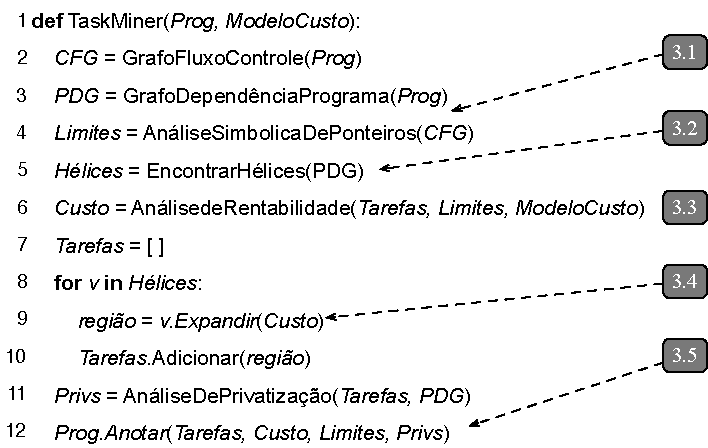
\includegraphics[width=1\columnwidth]{images/alg_main}
\caption{Os principais passos do algoritmo do TaskMiner.}
\label{fig:alg_main}
\end{center}
\end{figure}

A Figura~\ref{fig:alg_main} descreve o algoritmo executado pela ferramenta {\Taskminer}. 
Ele utiliza conceitos  como
o grafo de dependências ~\cite{Ferrante87} e o 
grafo de fluxo de controle~\cite{Kildall73}. {\Taskminer}
identifica tarefas em programas estruturados que podem
ser particionados em regiões \textit{hammock}
\cite{Ferrante87}.

\begin{Definicao} [Região \textit{hammock}]
\label{def:hammock}
Um grafo de fluxo de controle $G$ é um grafo direcionado com um nó de entrada
$s$ e um nó de saída $x$. Uma região \textit{hammock} $G'$ é um subgrafo de $G$ com um nó $h$ que {\em domina}
\footnote{Um nó $n_1 \in G$ domina outro nó
$n_2 \in G$ se todo caminho de  $S$ até $n_2$ atravessa $n_1$.
Inversamente, $n_1$ pós-domina $n_2$ se todo caminho de $n_2$ até $x$ deve passar por $n_1$.} os outros nós em $G$.
Além disso, existe um nó $w \in G$, $w \notin G'$, tal que $w$ {\em pós-domina} todo nó em $G'$. Nessa definição,
$h$ é o nó de entrada e $w$ é o nó de saída de $G'$.  
\end{Definicao}

\begin{Definicao} [Tarefa]
\label{def:task}
Em um programa $P$, uma tarefa $T$ é uma tupla $(G', M_i, M_o)$ formada
por uma região \textit{hammock} $G'$ e dois conjuntos $M_i$ e $M_o$, dados de memória lidos e escritos por $T$, respectivamente.
\end{Definicao}

Regiões de memória são descritas por variáveis do programa ou ponteiros com intervalos derrefenciáveis.
Sejam duas tarefas $T_1 = (G_1, M_{i1}, M_{o1})$ e $T_2 = (G_2, M_{i2}, M_{o2})$, 
se $M_{o1} \cap M_{i2} \neq \emptyset$ então $T_2$ {\em depende} de $T_1$. Se um programa $P$ está particionado em um 
conjunto de $n$ tarefas, então ele deve respeitar a Definição \ref{def:corretude} para ser considerado correto:

\begin{Definicao} [Corretude]
\label{def:corretude}
Um conjunto $T$ de $n$ tarefas é uma paralelização correta de um programa $P$ se:
\begin{compactenum}
\item $T$ não contém dependências cíclicas;
\item A execução das tarefas em $T$ em qualquer ordem determinada pelas relações de dependência devem resultar
identicamente à execução sequencial de $P$.
\end{compactenum}
\end{Definicao}

Abaixo há um exemplo de como as regiões de memória são marcadas em uma anotação de tarefa.
Considere-se duas tarefas $T_{\mathit{foo}} = (\mathsf{foo}, \{\mathsf{v[i - 1]}\},
\{v[i]\})$ e $T_{\mathit{bar}} = (\mathsf{bar}, \{v[i]\}, \{\})$. Dependências são identificadas na cláusula \textit{depend}. 
Nesse exemplo, cada região \textit{hammock} é constituída por uma chamada de função:

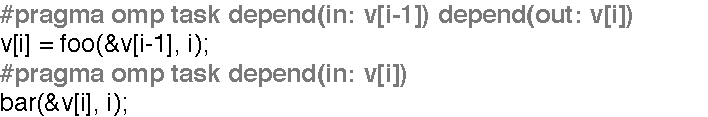
\includegraphics[width=1\columnwidth]{images/ex_depends}

{\Taskminer} utiliza OpenMP 4.5 para explorar o paralelismo de tarefas. Detalhes da sintaxe e semântica
das anotações do OpenMP estão publicamente disponíveis\footnote{``Summary of OpenMP 4.5 C/C++ Syntax", disponibilizado
pelo grupo OpenMP}. As anotações utilizadas são:
%
\begin{compactitem}
\item \textsf{parallel}: compõe um time de \textit{threads}
para executar a região anotada.
\item \textsf{single}: especifica uma região que deve ser executada
por apenas uma \textit{thread}.
\item \textsf{task}: cria uma nova tarefa.
\item \textsf{taskwait}: define um ponto de sincronização.
\end{compactitem}
%
Algumas dessas anotações são associadas a uma lista de cláusulas, a seguir:
\begin{compactitem}
\item \textsf{default([shared/private])}: indica se a variável é compartilhada ou replicada
entre tarefas.
\item \textsf{untied}: indica se uma tarefa não está associada à uma única \textit{thread},
permitindo ao ambiente balancemanto.
\item \textsf{depend}($\mathit{in}/\mathit{out}/\mathit{inout}$): determina se um dado é lido, escrito
ou ambos, explicitando as dependências entre as tarefas.
\item \textsf{if}({\em condição}): define uma condição para que aquela anotação seja executada.
\end{compactitem}

\subsection{Encontrando limites simbólicos}
\label{sec:sra}

Para produzir uma anotação que criará uma tarefa $T = (G, M_i, M_o)$,
deve-se determinar as regiões de memória $M_i$ que $T$ lê, e as regiões
$M_o$ em que $T$ escreve. Para tal, recorre-se à análise de limites simbólicos.
 
A instrução \textsf{U[i] += V[i*N + j]} na linha 9 da Figura~\ref{fig:ex_Regions}
contém dois acessos à memória: \textsf{U[i]} e
\textsf{V[i*N + j]}.
 O primeiro cobre a região de memória $[\mathtt{\&}\mathsf{U},
\mathtt{\&}\mathsf{U} + (\mathsf{M} - 1) \times \mathsf{sizeof}(\mathtt{int})]$.
O segundo cobre a região 
$[\mathtt{\&}\mathsf{V} + \mathsf{N} \times \mathsf{sizeof}(\mathtt{int}), \mathtt{\&}\mathsf{V} + ((\mathsf{i} \times \mathsf{M} + j) - 1) \times \mathsf{sizeof}(\mathtt{int})]$.
Não há código na Figura~\ref{fig:ex_Regions} que dependa do laço nas linhas 8-10.
Portanto, uma anotação de tarefa deve considerar apenas a dependência de entrada, ou seja,
o acesso à \textsf{V}. A cláusula \textsf{depend} na linha 6 contém uma referência
a essa região.

\begin{Definicao} [Análise de Limites Simbólicos]
\label{def:limites}
É uma forma abstrata de interpretação que associa uma variável inteira $v$
a um intervalo simbólico $R(v) = [l, u]$ em que $l$ e $u$ são expressões simbólicas.
Uma expressão simbólica $E$ é definida pela gramática abaixo, em que $s$ é um 
símbolo do programa:
\renewcommand{\arraystretch}{0.9}
\[
\begin{array}{rcl}
E & ::= & z \ \ | \ \ s \ \ | \ \ E + E \ \ | \ \ E \times E \ \ | \ \  \mbox{min}(E, E) \ \ | \\
&  & \mbox{max}(E, E) \ \ | -\infty \ \ | \ \ +\infty
\end{array}
\]
\end{Definicao}

Exemplos de símbolos de programa incluem variáveis globais, argumentos de função e retornos de
funções externas. A técnica
escolhida para as análises do {\Taskminer} é a mesma do compilador \dawn{} \cite{Mendonca17}.
Essa implementação é sólida o suficiente para lidar com toda a linguagem C99, sempre termina
e executa em tempo quadrático no número de variáveis do programa.

Por exemplo, se aplicada à Figura~\ref{fig:ex_Regions}, a análise de limites resulta em 
$R(\mathsf{i}) = [0, \mathsf{N} - 1]$, e $R(\mathsf{j}) = [0, \mathsf{M} - 1]$.
O acesso à memória \textsf{V[i*N + j]} na linha 9, combinado a essa informação, fornece
a região simbólica que aparece na anotação da linha 6 na Figura~\ref{fig:ex_Regions}.

\subsection{Mapeando regiões em tarefas}
\label{sub:identification}

% Windmills and vanes
Uma {\em tarefa candidata} é um conjunto de instruções que podem executar paralelamente.
Para identificá-las, {\Taskminer} faz uso do {\em Grafo de Dependências}. 

\begin{Definicao} [Grafo de Dependências (PDG) ~\cite{Ferrante87}]
\label{def:pdg}
Dado um programa
$P$, seu PDG contém um vértice para cada instrução $s \in P$. Existe uma aresta de 
$s_1$ a $s_2$ se o último depende do primeiro. $s_2$ tem uma dependência de dados de $s_1$
se lê dados que $s_1$ escreve. $s_2$ tem uma dependência de controle de $s_1$ se $s_1$ controla
a execução de $s_2$ a partir do resultado de um \textit{branch}, por exemplo.
\end{Definicao}

Tarefas candidatas são \textbf{hélices em moinhos}. {\em Moinhos} são uma família de grafos ~\cite{Rideau08}.
Moinhos existem como subgrafos do grafo de dependências. 

\begin{Definicao} [Moinho]
\label{def:moinho}
Um moinho é um grafo $G_w = G_c \cup G_{v1} \cup \ldots \cup G_{vn}$
formado por componentes fortemente conexos $G_c$ (centro do Moinho) e $n$ componentes, não necessariamente
fortes, $G_{vi}$ chamados de hélices, tais que:
\begin{compactenum}
\item para qualquer ordenação topológica de $G_w$, e os nós $n_c \in G_c$,
$n_v \in G_{vi}$, $n_c$ está à frente de $n_v$;
\item para qualquer $i$ e $j$, $1 \leq i < j \leq n$, $G_{vi}$ e $G_{vj}$ não
compartilham vértices (portanto, compartilhar arestas também é impossível).
\end{compactenum}
\end{Definicao}

\begin{figure}[h]
\begin{center}
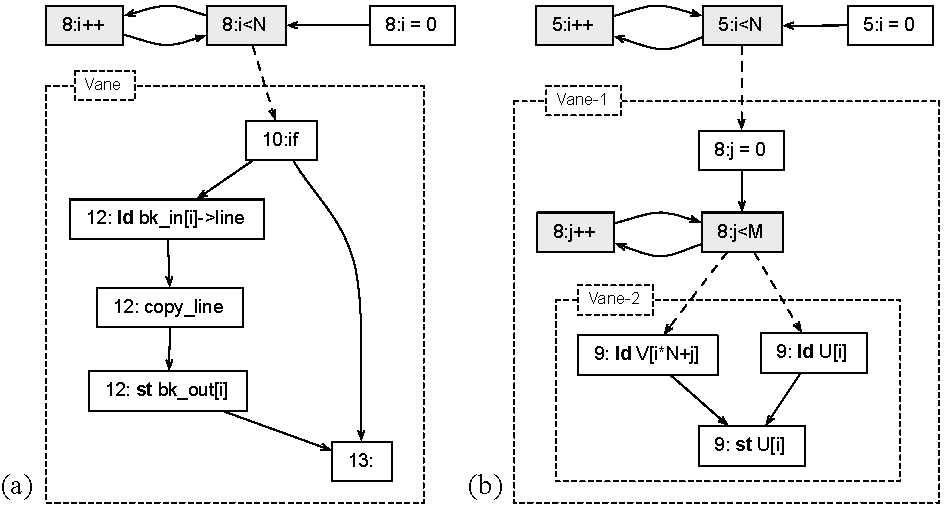
\includegraphics[width=1\columnwidth]{images/ex_windmill}
\caption{Exemplos de grafos de dependências. Nós que formam centros de moinhos
são coloridos de cinza. Arestas sólidas representam dependências de dados; arestas pontilhadas
dependências de controle. Hélices de moinhos aparecem dentro de retângulos pontilhados.
Na imagem, vemos o grafo para a Figura~\ref{fig:ex_Regions} em (b).}
\label{fig:ex_windmill}
\end{center}
\end{figure}

A Figura ~\ref{fig:ex_windmill} mostra dois grafos de dependências e seus
moinhos. A estrutura de moinhos naturalmente evidencia tarefas candidatas.
Hélices correspondem a partes do programa que tem alta probabilidade de serem
executadas diversas vezes, pois surgem de um laço: o centro do moinho. Duas execuções
de uma mesma hélice podem ser paralelas. Esta é uma propriedade do PDG e também uma 
das motivações originais para este trabalho. Essas duas execuções podem ser vistas como duas instâncias
da mesma estrutura: a hélice, partindo do mesmo centro do moinho. 
Uma ordenação topológica desse grafo não impõe
ordem entre as duas hipotéticas réplicas da mesma hélice.

Moinhos possuem propriedades estruturais para identifica-\c{c}\~{a}o de tarefas e são encontrados
em uma simples busca em profundidade no PDG. Entretanto, nem todo moinho
evidencia tarefas rentáveis. Ainda, alguns moinhos não podem ser anotados devido à inabilidade 
da análise de ponteiros em encontrar limites de acesso à memória. As próximas seções tratam desses
problemas.

\subsection{Estimando a lucratividade de tarefas}
\label{sub:profit}

O benefício de tarefas depende de dois fatores: custo de execução e paralelismo.
A dificuldade surge em encontrar o ponto mediano entre tarefas grandes e tarefas pequenas.
Tarefas muito pequenas são mais paralelas, pois tendem a ter menos dependências. 
Entretanto, se uma tarefa é muito pequena, 
então os ganhos de performance são eclipsados pelo custo do ambiente de execução
em manter essa tarefa ativa, e o paralelismo extra não compensa.
Por outro lado, se tarefas são muito grandes, então não há paralelismo: 
tarefas individuais executarão sequencialmente.
{\Taskminer} marca como tarefa as hélices que são maximais 
em termos de custo de execução, ou seja, as menores hélices
que estão acima do custo de execução no ambiente escolhido.

O tamanho de uma tarefa é dado pelo seu número de instruções. A mesma região de um programa
pode levar à criação de tarefas com tamanhos diferentes. 
Portanto, o tamanho real de uma tarefa só é conhecido ao final 
de sua execução. Para julgar a rentabilidade de uma tarefa,
deve-se aproximar esse tamanho
estaticamente. Assim, define-se a noção de {\em Trabalho Estático Estimado}:

% Explain the tension between large and small tasks.
\begin{Definicao}[Trabalho Estático Estimado (TEE)]
\label{def:swe}
Seja $G = G_1 \cup G_2 \cup \ldots \cup G_n$ uma partição de um grafo de controle
de um $G$ em $n$ regiões {\em hammock} {\em disjuntas}.
Trabalho Estático Estimado ($W(G)$) é definido como um número real não negativo,
tal que $W(G) = W(G_1) + W(G_2) + \ldots + W(G_n)$.
\end{Definicao}

O objetivo é obter um $TEE$ próximo ao comportamento dinâmico dos programas.
A heurística escolhida para este trabalho utiliza a análise de limites
descrita na Seção \ref{sec:sra} para inserir informações dinâmicas estaticamente
através da construção de expressões simbó-licas que representam o número de iterações
de laços. Essas expressões são inseridas em condicionais para a criação da
tarefa, como na linha 7 da Figura \ref{fig:ex_Regions}.

\begin{figure}[t!]
\begin{small}
\begin{eqnarray*}
\begin{tabular}{lc}
\textsc{[Instr]} &
W(\mbox{instr}) = \mbox{TEE, como especificado.}
\\\\
\textsc{[Seq]} &
\inferrule{W(S_1) = w_1 \\ W(S_2) = w_2}{W(S_1;S_2;) = w_1 + w_2}
\\\\
\textsc{[Branch]} &
\inferrule{W(S_1) = w_1 \\ W(S_2) = w_2 \\ W(S_3) = w_3}
{W(\mbox{if}(S_1) \ S_2; \ \mbox{else} \ S_3;) = w_1 + \mbox{max}(w_2, w_3)}
\\\\
\textsc{[LoopInf]} &
\inferrule{W(S_1) = w_1 \\ W(S_2) = w_2 \\ \mathit{Iter}(S_1) = \infty}
{W(\mbox{while} (S_1) \ S_2;) = 10 \times (w_1 + w_2)}
\\\\
\textsc{[LoopExp]} &
\inferrule{W(S_1) = w_1 \\ W(S_2) = w_2 \\ \mathit{Iter}(S_1) = E}
{W(\mbox{while} (S_1) \ S_2;) = E \times (w_1 + w_2)}
\end{tabular}
\end{eqnarray*}
\end{small}
\caption{\label{fig:swe}Estimando o custo das tarefas.}
\end{figure}

% Explain how we use symbolic information to compute costs.
As regras declarativas da Figura~\ref{fig:swe} esboçam as heurísticas
utilizadas para computar o TEE para uma região {\em hammock} $S$.
A regra \textsc{LoopInf} aplica-se a laços cujo número de iterações não
pode ser limitado por uma expressão simbólica computada estaticamente.
Assume-se que laços executam ao menos 10 vezes~\cite{Wu94}.
A regra \textsc{LoopExp} representa laços que não podem ser analisados 
com a análise de limites simbólicos. A função auxiliar $\mathit{Iter}(S)$ 
retorna uma expressão simbólica que representa a variedade de valores
cobertos pelo código em $S$ que controla o número de iterações do laço.

\paragraph{O Modelo de Custo.}
O {\Taskminer} recebe um modelo de custo como parâmetro.
Um modelo de custo é uma coleção de parâmetros que determinam o impacto
da criação e manuten-\c{c}\~{a}o de tarefas em uma determinada arquitetura.
A literatura lista técnicas analíticas e empíricas
para a construção do modelo~\cite{Poesia17}. 
Para os experimentos descritos na Seção ~\ref{sec:eval}, utilizou-se constantes
relacionadas à criação de {\em threads} em uma determinada arquitetura. Por exemplo,
a criação de tarefas foi estimada em 500 ciclos para a arquitetura em que os experimentos
foram realizados.

% Discuss the expansion algorithm.
\subsection{Expansão de tarefas}
\label{sub:expansion}

Expansão de tarefas consiste em encontrar a menor tarefa que é grande o suficiente
para compensar o custo de criação de {\em threads}. A Figura \ref{fig:expand_alg}
mostra o algoritmo de expansão. Inicia-se o algoritmo atribuindo \textsf{REGIÃO\_PAI} a
um grafo {\em hammock} $H$ que corresponde a uma hélice em um moinho $W$.
A decomposição {\em hammock} de um programa estruturado é uma árvore~\cite{Ferrante87},
em que os vértices representam grafos {\em hammock}.
$H_1$ é filho de $H_2$ na árvore se:
(i) $H_1 \subset H_2$, e (ii) para qualquer 
nó $H_x$, se $H_1 \subset H_x$ então $H_2 \subset H_x$.
Nese contexto, $H_2$ é {\em pai} de $H_1$.

\begin{figure}[h]
\begin{center}
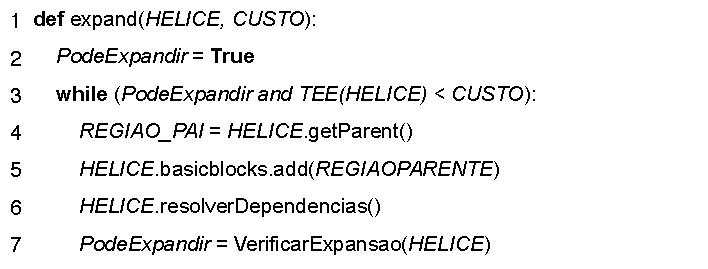
\includegraphics[width=1\columnwidth]{images/expand_alg}
\caption{Descoberta de tarefas em regiões {\em hammock}.
\textsf{CUSTO} é o custo de criação e escalonamento de {\em threads}.}
\label{fig:expand_alg}
\end{center}
\end{figure}

A cada nova expansão, checa-se se a expansão é válida. A expansão é válida se:
(i) \textsf{HÉLICE} está contida em um moinho $W$;
(ii) as regiões de memória em \textsf{HÉLICE} podem ser analisadas de acordo com
a Seção \ref{sec:sra};
(iii) \textsf{HÉLICE} não depende de uma outra hélice no mesmo moinho $W$.

\begin{figure}[h]
\begin{center}
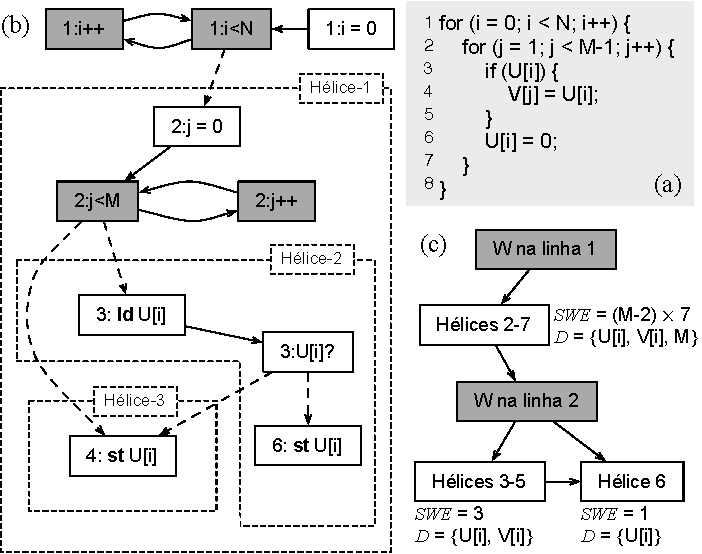
\includegraphics[width=1\columnwidth]{images/ex_expansion}
\caption{(a) Exemplo de laço duplamente aninhando analisado pelo {\Taskminer}.
(b) O Grafo de Dependências do programa.
(c) A decomposição desse laço em moinhos e hélices. $D$ é o conjunto de variáveis
das quais as hélices dependem.}
\label{fig:ex_expansion}
\end{center}
\end{figure}

O programa na Figura~\ref{fig:ex_expansion} (a) contém dois moinhos.
O primeiro consiste do laço da linha 1. O outro, aninhado, é o laço da linha 2.
As hélices que surgem desses moinhos estão evidenciadas na Figura~\ref{fig:ex_expansion} (b).
Na Figura, há 3 tarefas candidatas, cada uma formada por uma hélice.
Para encontrá-las, aplica-se a função de expansão (Fig.~\ref{fig:expand_alg})
nas hélices mais internas: \textsf{Hélice-2} pode ser expandida para incluir \textsf{Hélice-3}.

A expansão ocorre até o limite definido pelo \textsf{CUSTO}, que é determinado pelo modelo de custo
da Seção~\ref{sub:profit}. Se a lucratividade é menor que este custo, então
a criação da tarefa não é desejável. Se a tarefa é expandida demais, 
há perda de paralelismo: o código executa sequencialmente. Portanto, determinar o \textsf{CUSTO}
é essencial para o desempenho do {\Taskminer}.

\subsection{Anotando o código fonte}
\label{sub:ir}

As análises deste artigo foram implementadas na representa\c{c}\~{a}o intermediária (R.I.)
do LLVM devido à facilidade do uso de análises como evolução escalar~\cite[p.18]{Grosser12} e outras.
Porém, as anotações são inseridas em código fonte C, então grande
parte deste trabalho é o mapeamento de informações da R.I. do LLVM de volta
para código C.

% Explain machinery: scope tree and simplification
\noindent
\textbf{Árvore de escopos:}
A árvore de escopos é uma estrutura utilizada pelo {\Taskminer} para mapear regiões {\em hammock} em construtos C, como blocos
\textsf{while} e \textsf{if-then-else}. Cada nó nesta árvore contém {\em metadados}
provenientes de informação de depuração obtida durante a compilação para R.I.
É possível achar o número da linha relacionada à cada nó na árvore de escopos, permitindo
ao {\Taskminer} a anotação das regiões {\em hammock} no código fonte de maneira precisa.

\paragraph{Limitando a criação de tarefas recursivas}
Para evitar a criação excessiva de tarefas pequenas, {\Taskminer} dá a opção
aos usuários de limitar a criação de tarefas. Por exemplo, \textsf{./Taskminer -r 12} limita o número
de tarefas criadas a um total de 12 tarefas. Essa solução é implementada na fase de anotação. 
Essa solução traz claros benefícios em benchmarks recursivos, como mostra-se na Seção \ref{sec:eval}. 
A variável, chamada de \textsf{taskminer\_depht\_cutoff} na Figura
\ref{fig:ex_cutoff}, é global e ligada estaticamente. 
No começo de cada função recursiva
esta variável é incrementada para indicar a criação de uma nova tarefa, 
e decrementada ao sair da função.
A Figura~\ref{fig:ex_cutoff} ilustra a limitação de tarefas 
durante invocação recursiva.
O parâmetro \textsf{PROFUNDIDADE\_MAX}
é determinado pelo usuário.

Embora simples, a medida implementada é genérica o suficiente para lidar com 
tarefas difíceis de se
limitar simbolicamente. 
Há outras formas de limitar o número de tarefas recursivas~\cite{Iwasaki16}.
Futuramente, 
pretende-se explorar melhores maneiras de
limitar criação de tarefas pequenas.

\section{Avalia\c{c}\~{a}o Experimental}
\label{sec:eval}

{\Taskminer} foi implementado em LLVM 3.9. Os experimentos
foram executados em uma máquina de 12 núcleos 64-bits Intel(R) Xeon(R) CPU E5-2620, 2.00GHz, com 32K de cache L1, 256K de cache L2 e 15M de cache L3, e 15Gb de memória RAM. Utilizou-se OpenMP 4.5.

\subsection{Desempenho}
\label{sub:performance}

\begin{figure}[b!]
\begin{center}
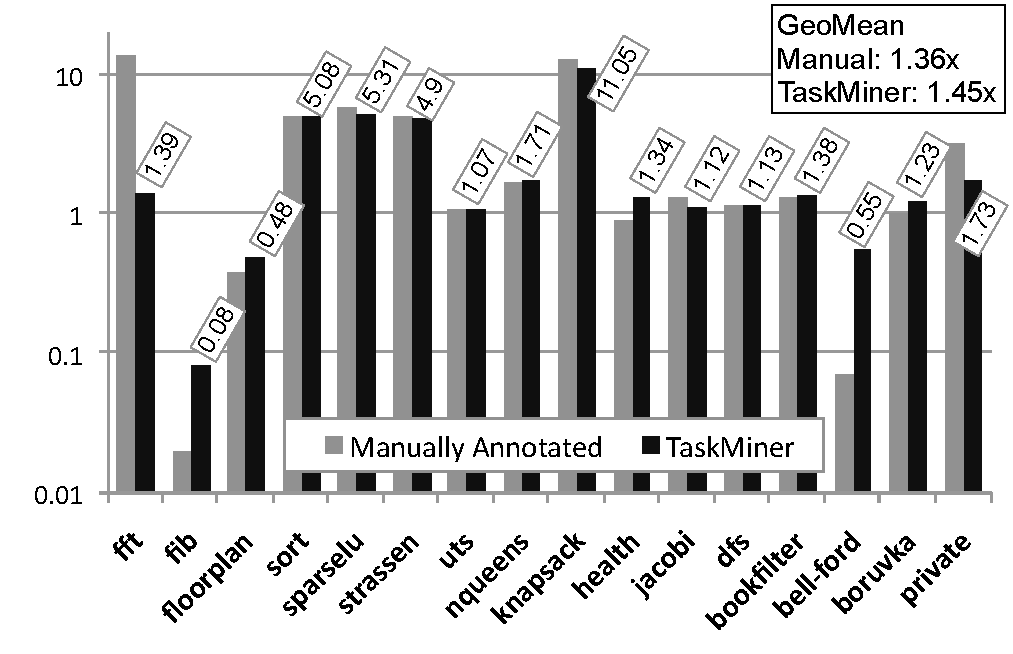
\includegraphics[width=1\columnwidth]{images/TM_Performance}
\caption{Comparações de performance. Anotações automáticas comparam-se favoralmente a intervenções
manuais, e levam a ganhos de desempenho. No eixo y, o ganho de desempenho de cada versão anotada
pelo {\Taskminer} e de cada versão anotada manualmente. Os números nas caixas representam
o crescimento em velocidade obtido.}
\label{fig:TM_Performance}
\end{center}
\end{figure}

A Figura~\ref{fig:TM_Performance} compara o tempo de execução de programas produzidos
pelo {\Taskminer} contra versões originais dos mesmos programas anotados manualmente.
Os {\em benchmarks} utilizados neste experimento são do \textsf{BSC-Bots}~\cite{Duran09} 
e do \textsf{Swan}~\cite{Moreira17}.
Ambos vêm com versões sequenciais e paralelas (anotadas manualmente). Os códigos foram compilados
com gcc-6.

As versões anotadas pelo \Taskminer{} foram mais velozes que as sequenciais em 13 dos 16 programas.
A maioria são algoritmos Dividir \& Conquistar clássicos como multiplicação de matrizes de \textsf{Strassen},
 \textsf{knapsack} (Problema da Mochila) e \textsf{fft} (Transformada Rápida de Fourrier). Em 6 deles, as versões automáticas foram próximas e até
levemente superiores às versões anotadas manualmente. Em 3, \Taskminer{} produziu versões piores que
as versões sequenciais: \textsf{fib}, \textsf{floorplan} e \textsf{bell-ford}. Ainda assim, produziu versões
mais rápidas que as anotadas manualmente. Uma inspeção de \textsf{bell-ford} indica que a versão
paralelizada manualmente dispara um número grande tarefas pequenas. O modelo de custo
do \Taskminer{} poda a criação de tarefas pequenas, mas não o suficiente para vencer o desempenho
da versão sequencial. Este experimento demonstra que \Taskminer{} pode trazer
ganhos consideráveis se comparados às versões sequenciais e manualmente anotadas.

Além disso, destaca-se o fato de que as anotações do \Taskminer{} levaram resultados próximos às anotações manuais. Dessa forma, \Taskminer{} retira do programador o fardo de inserir as anotações manualmente.

%OPTIMIZATIONS
%Here, we show the results on two big optimizations: recursion depth and cost model.
%We can use the same benchmarks as above.
\subsection{Otimizações}
\label{sub:optimizations}

\begin{figure}[b!]
\begin{center}
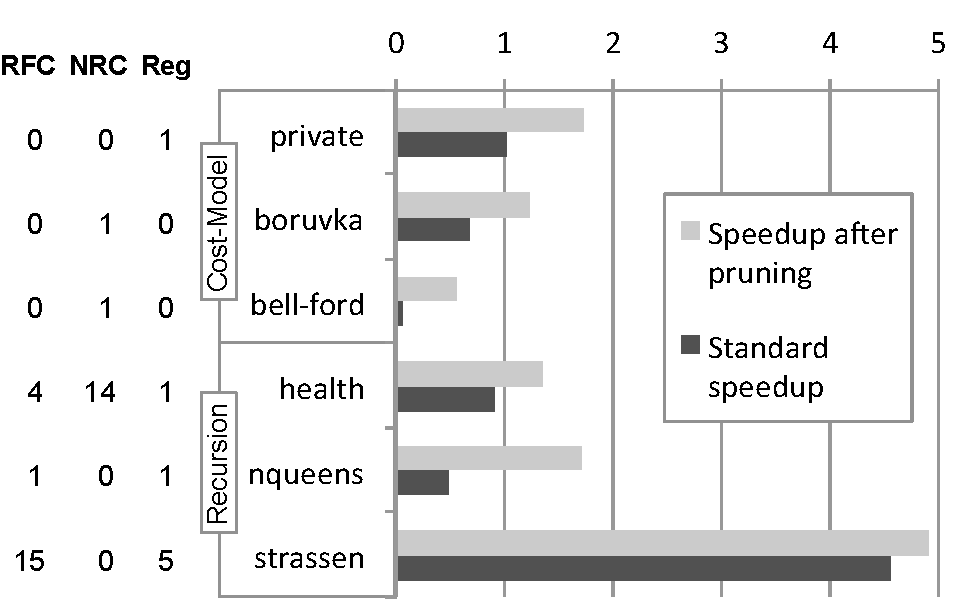
\includegraphics[width=1\columnwidth]{images/Optimizations}
\caption{Benefícios de limitar a criação de tarefas. (Secs.~\ref{sub:profit} e ~\ref{sub:ir}).
\textbf{CFR}: tarefas criadas em \underline{C}hamadas de \underline{F}unções \underline{R}ecursivas.
\textbf{CNR}: tarefas interprocedurais criadas ao redor de \underline{C}hamadas  \underline{N}ão-\underline{R}ecursivas.
\textbf{Reg}: tarefas envolvendo \underline{Reg}iões, sem chamadas de função.}
\label{fig:Optimizations}
\end{center}
\end{figure}

Ambas as formas de 
otimizar a criação de tarefas descritas neste artigo são baseadas na ideia de 
{\em poda}: evita-se a criação de tarefas consideradas não-lucrativas. 
Limita-se a criação de tarefas ditas não lucrativas de acordo com o modelo de custo, 
conforme explicado na 
Seção~\ref{sub:profit}; e limita-se a criação de tarefas muito profundas na pilha de recursão, 
como descrito na Seção~\ref{sub:ir}. A Figura~\ref{fig:Optimizations} ilustra os benefícios dessas duas técnicas,
presentes em 6 dos benchmarks vistos anteriormente (sec ~\ref{sub:performance}).

Em 3 benchmarks, \textsf{private}, \textsf{boruvka} e
\textsf{bellman-ford}, o modelo de custo evita a criação de tarefas em laços que inicializam estruturas de dados.
Por exemplo, o laço a seguir, na linha 75 do programa \textsf{bellmanford.c}, seria paralelizado pelo
\Taskminer{}, caso o modelo de custo o marcasse como lucrativo:

\begin{verbatim}
  for (long unsigned i = 0; i < N; i++)
    for (long unsigned j = 0; j < N; j++)
      *(G + i * N + j) = rand();
\end{verbatim}

A limitação de tarefas recursivas (Sec.~\ref{sub:ir}), embora simples,
é efetiva em eliminar o excesso de tarefas pequenas. 
A Figura~\ref{fig:Optimizations} mostra esse impacto em três programas: \textsf{health}, \textsf{nqueens} e
\textsf{strassen}. Estes programas foram projetados para ilustrar paralelismo
em paradigma Dividir \& Conquistar, e contém muitas chamadas
recursivas. A poda em níveis mais altos da árvore de recursão leva a bons ganhos de desempenho. 
Caso não houvesse essa otimização de poda, então perda de desempenho seria observada
em  \textsf{health} e \textsf{nqueens}, provando que as otimizações são eficazes e melhoram
a qualidade do código gerado pelo \Taskminer{}.

%VERSATILITY
%The goal here is to show that TaskMiner is a versatile tool, capable of finding many types of task parallelism in the code. 
%And the types of tasks that are going to be mined can be easily set, should the programmer ever desires to.
\subsection{Versatilidade}
\label{sub:versatility}

Os benchmarks das seções anteriores foram projetados especialmente para o estudo de 
paralelismo irregular. Para determinar se o \Taskminer{} consegue encontrar paralelismo 
em programas comuns, executou-se o mesmo sobre 219 programas C disponíveis
na suíte de testes do LLVM, e comparou-se o desempenho da versão anotada automaticamente pelo
\Taskminer{} com a versão original sequencial. 
\Taskminer{} anota um programa se:
(i) consegue encontrar limites simbólicos para todos os acessos à memória que ocorrem em uma hélice; e
(ii) a hélice é ampla o suficiente para pagar pelo custo de criação de tarefas no ambiente de execução.
Sob esses termos, descobriu-se tarefas em 63 desses programas. A Figura~\ref{fig:TM_Versatility} relaciona
o número de tarefas ao número de instruções em 30 dos maiores programas utilizados.
Como demonstrado neste experimento,
\Taskminer{} é capaz de anotar um número não trivial de benchmarks reais.

\begin{figure}[htb]
\begin{center}
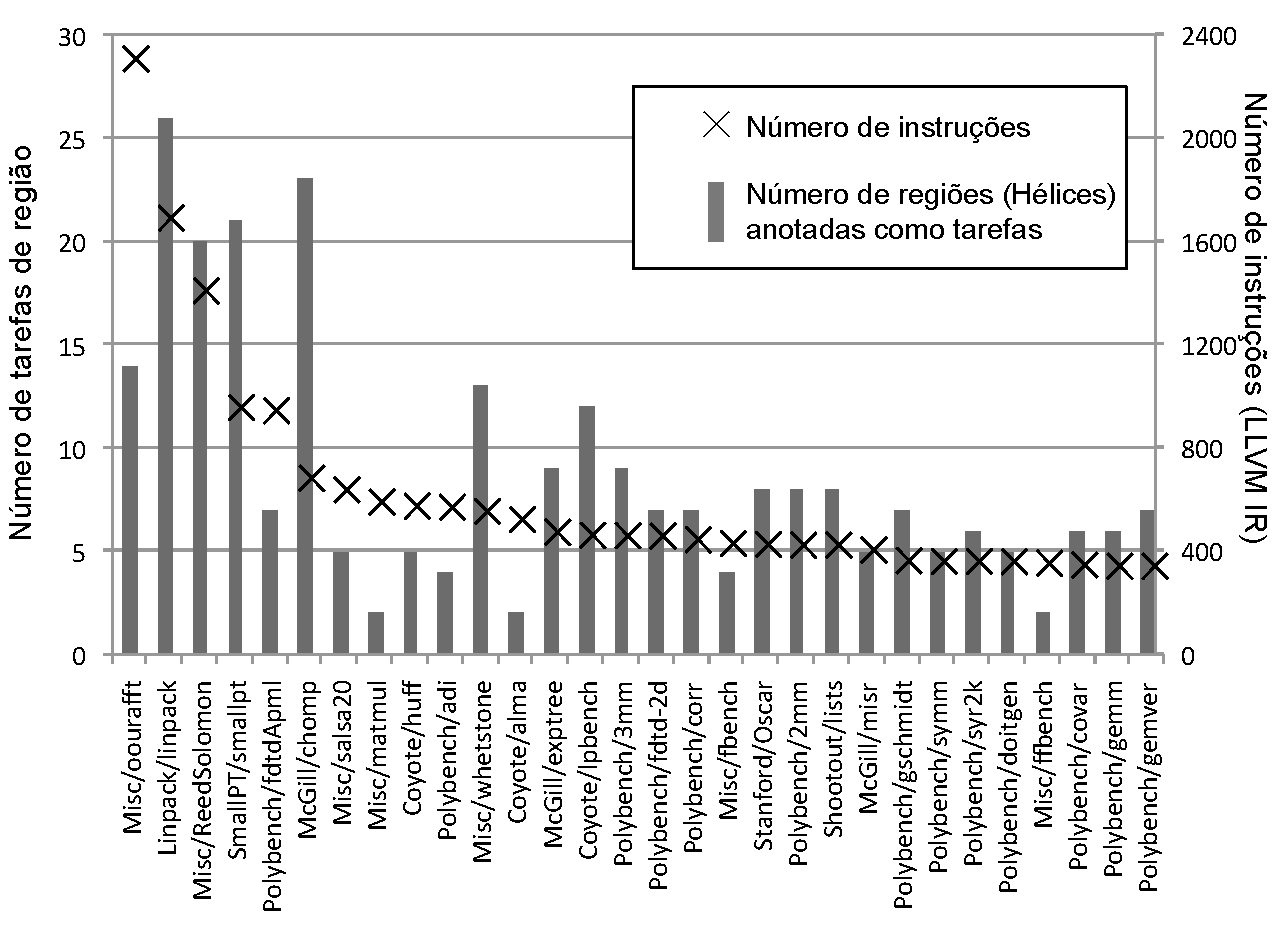
\includegraphics[width=1\columnwidth]{images/TM_Versatility}
\caption{Relação entre o número de regiões de tarefas e tamanho do programa.
Cada programa é um arquivo C completo.}
\label{fig:TM_Versatility}
\end{center}
\end{figure}

Dos benchmarks anotados, 27 não demonstraram aumento de desempenho em 
relação à versão sequencial,
pois as tarefas anotadas eram muito pequenas e pouco influenciaram na execução total do programa.
Em 17 deles, observou-se perda de velocidade: neste caso, interações entre estruturas de dados
forçaram o ambiente de execução do OpenMP a serializar a execução das tarefas. 
Essas perdas foram 
inferiores à 10\%. Porém, nota-se uma necessidade de desenvolver-se um modelo de custo mais robusto para evitar a geração de programas paralelos que sejam mais lentos que os originais sequenciais. Como trabalho futuro, pretende-se estudar melhores heurísticas para a estimativa do custo de uma tarefa, a fim de diminuir esse tipo de resultado. Observa-se que os programas que resultaram em perda de velocidade possuiam tarefas muito pequenas e irrelevantes proporcionalmente em relação ao resto do programa. É necessário um modelo de custo que considere também o tamanho do programa em relação às poções sequenciais e seus impactos no mesmo.

Obteve-se aumento de desempenho acima de 5\% em 19 programas. 
Em \textsf{Misc/lowercase}, o fator de crescimento foi acima de 3,5x, e em 3 casos, acima de 1.5x.
A Figura~\ref{fig:TM_GeneralProgs} mostra os 10 maiores acréscimos de desempenho obtidos pelo \Taskminer{}.
Enfatiza-se que esse experimento {\em não contou com nenhum tipo de intervenção humana}.
Portanto, \Taskminer{} é capaz de encontrar paralelismo automaticamente sem custo de programação.

\begin{figure}[t!]
\begin{center}
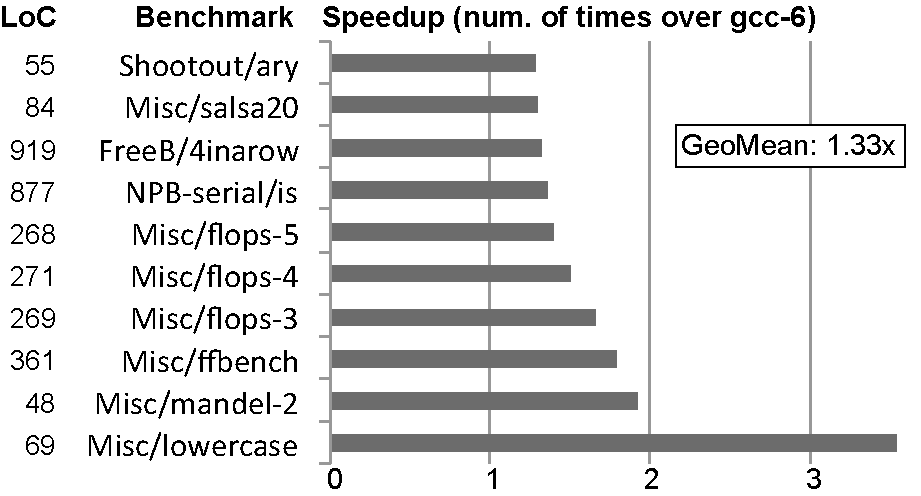
\includegraphics[width=1\columnwidth]{images/TM_GeneralProgs}
\caption{Melhorias de desempenho obtidas pelo \Taskminer{} quando aplicado à suíte de testes
do LLVM. Quanto maior a barra, maior o ganho de desempenho.
\textbf{LoC} significa ``Linhas de Código".}
\label{fig:TM_GeneralProgs}
\end{center}
\end{figure}


%{\Taskminer}'s versatility also arises in regards to the diversity of types of task parallelism that it
%can find in a program. Table \ref{tab:types} shows all types of tasks found in our main benchmarks.
%There are 3 types of tasks: recursive, which arises from vanes in Divide and Conquer
%algorithms; function call, which arises within loops that are not clearly parallel; and region, which 
%are similar to function calls, but instead are entire fragments of code within loops that can be executed in
%parallel. We provide the user complete decision power to mine for any type of tasks they wish when
%running our tool. 

%SCALABILITY
\section{Trabalhos Relacionados}
\label{sec:rw}

Compiladores modernos adicionaram suporte ao paralelismo de tarefas 
do OpenMP apenas recentemente. Uma implementação do \textsf{clang} com suporte a Tasks foi lançada em Março, 2014. Tal suporte foi integrado ao \textsf{gcc} em Abril do mesmo ano.
Uma vez que a infra-estrutura necessária para
a implementação de tarefas é nova, não existem ferramentas estáticas
além do {\Taskminer} capazes de anotar programas
automaticamente com diretivas de tarefas. Entretanto, existe muita pesquisa em paralelização automática de código.

Padrões de anotação de código baseados em diretivas conferem ao programador um modelo de programação paralela fácil de se utilizar. Extensões destes padrões baseadas em tarefas resultaram em  OpenMP 4.X,
StarSs \cite{planas:hpca:2009,
tejedor:hpdc:2011} e OmpSs \cite{bueno:icpp:2011}. Tais modelos vem com ferramentas que ajudam os programadores a achar as melhores anotações para seus códigos. Por exemplo, Tareador \cite{Ayguade15} permite ao programador, através de uma interface gráfica, a anotar código sequencial, permitindo assim a identificação de potenciais oportunidades de tarefas. Ao contrário do Tareador, este trabalho propõe uma abordagem que permite a inserção automática de anotações OpenMP em fragmentos relevantes de um programa sequencial.

As técnicas utilizadas neste trabalho para mapear regiões de programas em tarefas é similar às análises muito utilizadas em geração de código para máquinas de fluxo de dados. Programação de fluxo de dados foi originalmente proposto como um paradigma adequado ao paralelismo de tarefas \cite{agrawal:ipdps:2010,
gupta:micro:2011}. Este paradigma foi extendido com especificações para entrada e saída de tarefas em Cilk++ \cite{agrawal:ipdps:2010}, e mais tarde Cilk++ foi extendido com cláusulas de dependência para facilitar a projeção de padrões de paralelização \cite{vandierendonck:hotpar:2011}. O modelo, até então, apresentava um escalonador unificado baseado em paralelismo {\em fork-join} que permitia a execução de aplicações baseadas em tarefas. Outras abordagens também utilizaram grafos de fluxo de dados para explorar paralelismo, como tarefas de dados, nas quais o programador pode utilizar cláusulas de \textit{put} e \textit{await} para determinar os argumentos de uma tarefa antes de sua execução. Paralelismo de tarefas baseado em argumentos de funções também foi proposto para a determinação de dependências entre tarefas \cite{gupta:micro:2011}. Nota-se que os esforços listados focam-se em conceder ao programador as ferramentas para construir programas paralelos. A geração automática de programas paralelos simples não estava entre seus objetivos.

Muitos sistemas foram desenvolvidos para extrair paralelismo de tarefas a partir de programas sequenciais de maneira semi-automática. Exemplos incluem OSCAR (Optimally SCheduled Advanced multprocessoR), um compilador-paralelizador \cite{ishizaka:journal:2000}, MAPS (MPSoC Application Programming Studio) \cite{castrillon:tii:2013} e DiscoPoP (Discovery of Potential Parallelism) \cite{li:jss:2016}. Além de sistemas de paralelização, ferramentas como Paraver  \cite{paraver}, Aftermath~\cite{drebes:hipeac:2014}, DAGvis \cite{huynh:wvpa:2015}, e TEMANEJO
\cite{temanejo} foram projetadas para permitir análises de performance e visualização de programas em tarefas. 

Apesar dessas ferramentas ajudarem o programador a adaptar código para rodar em paralelo, elas não são completamente automáticas. Por exemplo, o trabalho que é mais próximo ao descrito neste artigo é o conjunto de análises estáticas propostas por Ravishankar {\em et al.} \cite{Ravishankar14}. O tipo de laços irregulares com os quais eles lidam é impressionante; porém, a falta de suporte a \textsf{OpenMP 4.X} ainda requer ao programador modificar código antes da paralelização. Nas palavras dos autores, ``{\em para todos os benchmarks e aplicações, todas as funções foram alinhadas, e arranjos de estruturas foram convertidos a estruturas de arranjos para uso em conjunto com o nosso protótipo}", de forma que o sistema modifica o código original para atingir o paralelismo desejado. \Taskminer{}, por outro lado, não modifica a sintaxe do programa sequencial original.

Em outro contexto, ferramentas foram desenvolvidas para inser-ção de anotações automáticas que expõe paralelismo de dados \cite{Wang2009}. Essas ferramentas, porém, além de explorarem outro tipo de paralelismo, não são completamente estáticas e automáticas como o \Taskminer{}.

\section{Conclus\~{a}o}
\label{sec:conc}

Este trabalho apresentou \Taskminer{}, uma ferramenta capaz de identificar automaticamente oportunidades de paralelismo de tarefas e anotá-las com diretivas OpenMP. \Taskminer{} implementa algoritmos de análise de código em representação intermediária do LLVM e contorna problemas clássicos no paralelismo irregular. \Taskminer{} prova-se eficiente e competitivo, sendo capaz de anotar programas não triviais e encontrar paralelismo escondido sem custo adicional. 

Embora já possa ser usado em produção de código paralelo, \Taskminer{} ainda apresenta espaço
para melhorias.
Em particular, \Taskminer{} implementa uma heurística simples demais para estimar o custo de uma tarefa.
Dada a sua simplicidade, essa heurística não é firme o suficiente para garantir a lucratividade de uma anotação. Como trabalho futuro, pretende-se implementar heurísticas de estimativa de custo que sejam mais precisas, para refinar o algoritmo do \Taskminer{}. Embora ainda sob constantes atualizações, uma versão inicial do
\Taskminer{} está online e disponível para uso acadêmico em \url{http://cuda.dcc.ufmg.br/taskminer/}.

\bibliography{references}

\end{document}
